\documentclass[12pt,a4paper,titlepage]{article}
\title{Sound Event Detection con la tecnica del “few-shot learning“} 
\author{Matteo Orlandini}
\date{\today}

\usepackage[english, italian]{babel} %the last declared language is the one used in the document
\usepackage[utf8]{inputenc}
\usepackage[T1]{fontenc}
\usepackage{booktabs} %toprule, midrule, bottomrule
\usepackage{subfig}
\usepackage{graphicx}
\usepackage{listings}
\usepackage{siunitx}
\usepackage{amsmath,amssymb}
\usepackage{xcolor}

\colorlet{punct}{red!60!black}
\definecolor{background}{HTML}{EEEEEE}
\definecolor{delim}{RGB}{20,105,176}
\colorlet{numb}{magenta!60!black}

\lstdefinelanguage{json}{
	basicstyle=\scriptsize,
	%numbers=left,
	tabsize=2,
	numberstyle=\scriptsize,
	stepnumber=1,
	numbersep=8pt,
	breaklines=true,
	frame=single,
	backgroundcolor=\color{background},
	literate=
	%*{0}{{{\color{numb}0}}}{1}
	%{1}{{{\color{numb}1}}}{1}
	%{2}{{{\color{numb}2}}}{1}
	%{3}{{{\color{numb}3}}}{1}
	%{4}{{{\color{numb}4}}}{1}
	%{5}{{{\color{numb}5}}}{1}
	%{6}{{{\color{numb}6}}}{1}
	%{7}{{{\color{numb}7}}}{1}
	%{8}{{{\color{numb}8}}}{1}
	%{9}{{{\color{numb}9}}}{1}
	%{:}{{{\color{punct}{:}}}}{1}
	{,}{{{\color{punct}{,}}}}{1}
	{\{}{{{\color{delim}{\{}}}}{1}
	{\}}{{{\color{delim}{\}}}}}{1}
	{[}{{{\color{delim}{[}}}}{1}
	{]}{{{\color{delim}{]}}}}{1},
 	morekeywords = {folder, reader_name, word, frequency, start, end, words, folders},
	keywordstyle=\bfseries\color{blue},
	commentstyle=\color{black},
	keepspaces=false,
	showspaces=false,
	showstringspaces=false,
}

\usepackage{color}
\definecolor{gray}{rgb}{0.4,0.4,0.4}
\definecolor{darkblue}{rgb}{0.0,0.0,0.6}
\definecolor{cyan}{rgb}{0.0,0.6,0.6}

\lstset{literate=
		{á}{{\'a}}1 {é}{{\'e}}1 {í}{{\'i}}1 {ó}{{\'o}}1 {ú}{{\'u}}1
		{Á}{{\'A}}1 {É}{{\'E}}1 {Í}{{\'I}}1 {Ó}{{\'O}}1 {Ú}{{\'U}}1
		{à}{{\`a}}1 {è}{{\`e}}1 {ì}{{\`i}}1 {ò}{{\`o}}1 {ù}{{\`u}}1
		{À}{{\`A}}1 {È}{{\'E}}1 {Ì}{{\`I}}1 {Ò}{{\`O}}1 {Ù}{{\`U}}1
		{ä}{{\"a}}1 {ë}{{\"e}}1 {ï}{{\"i}}1 {ö}{{\"o}}1 {ü}{{\"u}}1
		{Ä}{{\"A}}1 {Ë}{{\"E}}1 {Ï}{{\"I}}1 {Ö}{{\"O}}1 {Ü}{{\"U}}1
		{â}{{\^a}}1 {ê}{{\^e}}1 {î}{{\^i}}1 {ô}{{\^o}}1 {û}{{\^u}}1
		{Â}{{\^A}}1 {Ê}{{\^E}}1 {Î}{{\^I}}1 {Ô}{{\^O}}1 {Û}{{\^U}}1
		{ã}{{\~a}}1 {ẽ}{{\~e}}1 {ĩ}{{\~i}}1 {õ}{{\~o}}1 {ũ}{{\~u}}1
		{Ã}{{\~A}}1 {Ẽ}{{\~E}}1 {Ĩ}{{\~I}}1 {Õ}{{\~O}}1 {Ũ}{{\~U}}1
		{œ}{{\oe}}1 {Œ}{{\OE}}1 {æ}{{\ae}}1 {Æ}{{\AE}}1 {ß}{{\ss}}1
		{ű}{{\H{u}}}1 {Ű}{{\H{U}}}1 {ő}{{\H{o}}}1 {Ő}{{\H{O}}}1
		{ç}{{\c c}}1 {Ç}{{\c C}}1 {ø}{{\o}}1 {å}{{\r a}}1 {Å}{{\r A}}1
		{€}{{\euro}}1 {£}{{\pounds}}1 {«}{{\guillemotleft}}1
		{»}{{\guillemotright}}1 {ñ}{{\~n}}1 {Ñ}{{\~N}}1 {¿}{{?`}}1 {¡}{{!`}}1 
}

\lstdefinelanguage{XML}
{
	basicstyle=\tiny,	
	tabsize=2,
	frame=single,
	morestring=[b]",
	%morestring=[s]{>}{<},
	%morecomment=[s]{<?}{?>},
	stringstyle=\color{darkblue},
	identifierstyle=\color{cyan},
	keywordstyle=\bfseries\color{black},
	morekeywords={key, value, group, text, pronunciation, start, end}
	moreidentifier = {article, meta, link, prop, d, extra, t, s, n, ignored},
	backgroundcolor=\color{background},
	emph={key,end},          % Custom highlighting
	emphstyle=\bfseries\color{black},    % Custom highlighting style
	keepspaces=false,
	showspaces=false,
	showstringspaces=false,
	breaklines=true,         
	breakatwhitespace=false,  
}

\definecolor{maroon}{cmyk}{0, 0.87, 0.68, 0.32}
\definecolor{halfgray}{gray}{0.55}
\definecolor{ipython_frame}{RGB}{207, 207, 207}
\definecolor{ipython_bg}{RGB}{247, 247, 247}
\definecolor{ipython_red}{RGB}{186, 33, 33}
\definecolor{ipython_green}{RGB}{0, 128, 0}
\definecolor{ipython_cyan}{RGB}{64, 128, 128}
\definecolor{ipython_purple}{RGB}{170, 34, 255}


\lstdefinelanguage{iPython}{
	morekeywords={access,and,break,class,continue,def,del,elif,else,except,exec,finally,for,from,global,if,import,in,is,lambda,not,or,pass,print,raise,return,try,while},%
	%
	% Built-ins
	morekeywords=[2]{abs,all,any,basestring,bin,bool,bytearray,callable,chr,classmethod,cmp,compile,complex,delattr,dict,dir,divmod,enumerate,eval,execfile,file,filter,float,format,frozenset,getattr,globals,hasattr,hash,help,hex,id,input,int,isinstance,issubclass,iter,len,list,locals,long,map,max,memoryview,min,next,object,oct,open,ord,pow,property,range,raw_input,reduce,reload,repr,reversed,round,set,setattr,slice,sorted,staticmethod,str,sum,super,tuple,type,unichr,unicode,vars,xrange,zip,apply,buffer,coerce,intern},%
	%
	sensitive=true,%
	morecomment=[l]\#,%
	morestring=[b]',%
	morestring=[b]",%
	%
	morestring=[s]{'''}{'''},% used for documentation text (mulitiline strings)
	morestring=[s]{"""}{"""},% added by Philipp Matthias Hahn
	%
	morestring=[s]{r'}{'},% `raw' strings
	morestring=[s]{r"}{"},%
	morestring=[s]{r'''}{'''},%
	morestring=[s]{r"""}{"""},%
	morestring=[s]{u'}{'},% unicode strings
	morestring=[s]{u"}{"},%
	morestring=[s]{u'''}{'''},%
	morestring=[s]{u"""}{"""},%
	%
	% {replace}{replacement}{lenght of replace}
	% *{-}{-}{1} will not replace in comments and so on
	literate=
	{á}{{\'a}}1 {é}{{\'e}}1 {í}{{\'i}}1 {ó}{{\'o}}1 {ú}{{\'u}}1
	{Á}{{\'A}}1 {É}{{\'E}}1 {Í}{{\'I}}1 {Ó}{{\'O}}1 {Ú}{{\'U}}1
	{à}{{\`a}}1 {è}{{\`e}}1 {ì}{{\`i}}1 {ò}{{\`o}}1 {ù}{{\`u}}1
	{À}{{\`A}}1 {È}{{\'E}}1 {Ì}{{\`I}}1 {Ò}{{\`O}}1 {Ù}{{\`U}}1
	{ä}{{\"a}}1 {ë}{{\"e}}1 {ï}{{\"i}}1 {ö}{{\"o}}1 {ü}{{\"u}}1
	{Ä}{{\"A}}1 {Ë}{{\"E}}1 {Ï}{{\"I}}1 {Ö}{{\"O}}1 {Ü}{{\"U}}1
	{â}{{\^a}}1 {ê}{{\^e}}1 {î}{{\^i}}1 {ô}{{\^o}}1 {û}{{\^u}}1
	{Â}{{\^A}}1 {Ê}{{\^E}}1 {Î}{{\^I}}1 {Ô}{{\^O}}1 {Û}{{\^U}}1
	{œ}{{\oe}}1 {Œ}{{\OE}}1 {æ}{{\ae}}1 {Æ}{{\AE}}1 {ß}{{\ss}}1
	{ç}{{\c c}}1 {Ç}{{\c C}}1 {ø}{{\o}}1 {å}{{\r a}}1 {Å}{{\r A}}1
	{€}{{\EUR}}1 {£}{{\pounds}}1
	%
	{^}{{{\color{ipython_purple}\^{}}}}1
	{=}{{{\color{ipython_purple}=}}}1
	%
	{+}{{{\color{ipython_purple}+}}}1
	{*}{{{\color{ipython_purple}$^\ast$}}}1
	{/}{{{\color{ipython_purple}/}}}1
	%
	{+=}{{{+=}}}1
	{-=}{{{-=}}}1
	{*=}{{{$^\ast$=}}}1
	{/=}{{{/=}}}1,
	literate=
	*{-}{{{\color{ipython_purple}-}}}1
	{?}{{{\color{ipython_purple}?}}}1,
	%
	identifierstyle=\color{black}\ttfamily,
	commentstyle=\color{ipython_cyan}\ttfamily,
	stringstyle=\color{ipython_red}\ttfamily,
	keepspaces=false,
	showspaces=false,
	breaklines=true,
	showstringspaces=false,
	%
	rulecolor=\color{ipython_frame},
	frame=single,
	frameround={t}{t}{t}{t},
	framexleftmargin=6mm,
	numbers=left,
	numberstyle=\tiny\color{halfgray},
	%
	%
	backgroundcolor=\color{ipython_bg},
	%   extendedchars=true,
	basicstyle=\scriptsize,
	tabsize=2,
	keywordstyle=\color{ipython_green}\ttfamily,
	morekeywords={typeof, null, catch, switch, in, int, str, float, self, import, def, return, True, False, None},
	emph={read_json_file,write_json_file, exists, parse, getroot, basename, scandir, keys, Counter, append, sample},          % Custom highlighting
	emphstyle=\color{ipython_purple}\ttfamily,    % Custom highlighting style
}

%\usepackage[latin1]{inputenc} %l'ho messo io (Jacopo)
%inizio impostazioni bibliografia
\usepackage[autostyle,italian=guillemets]{csquotes} 
%autostyle adatta lo stile delle citazioni alla lingua corrente del documento;
%italian=guillemets racchiude automaticamente tra virgolette caporali
%i campi che prevedono le virgolette;
\usepackage[backend=biber, style=numeric, citestyle=numeric,maxcitenames=99,maxbibnames = 99]{biblatex}
%backend=biber dice a biblatex che s’intende usare Biber come motore bibliografico
%style:numeric Anno di pubblicazione: in fondo al riferimento.
%citestyle=numeric Riferimento: numerico ([1], [2], eccetera).
%fine impostazioni bibliografia

\usepackage{float}
\usepackage{hyperref}
\hypersetup{
%	bookmarks=true,         % show bookmarks bar?
	unicode=false,          % non-Latin characters in Acrobat’s bookmarks
	pdftoolbar=true,        % show Acrobat’s toolbar?
	pdfmenubar=true,        % show Acrobat’s menu?
	pdffitwindow=false,     % window fit to page when opened
	pdfstartview={FitH},    % fits the width of the page to the window
	%pdftitle={Relazione di Reti di Sensori Wireless per IOT},    % title
	pdfauthor={Matteo Orlandini},     % author
	pdfsubject= {Sound Event Detection con la tecnica del few-shot learning},   % subject of the document
	pdfcreator={Matteo Orlandini},   % creator of the document
	%pdfproducer={Producer}, % producer of the document
	pdfpagemode={UseOutlines},
	%bookmarksopen,
	pdfstartview={FitH},
	colorlinks=false,       % false: boxed links; true: colored links
	linkcolor={red},
	citecolor={green},
	urlcolor={cyan}
} 

\renewcommand{\lstlistingname}{Codice}

\addbibresource{Bibliografia.bib}

\newcommand{\CoverName}{Cover}

\begin{document}

\begin{titlepage}
	
	\centering
	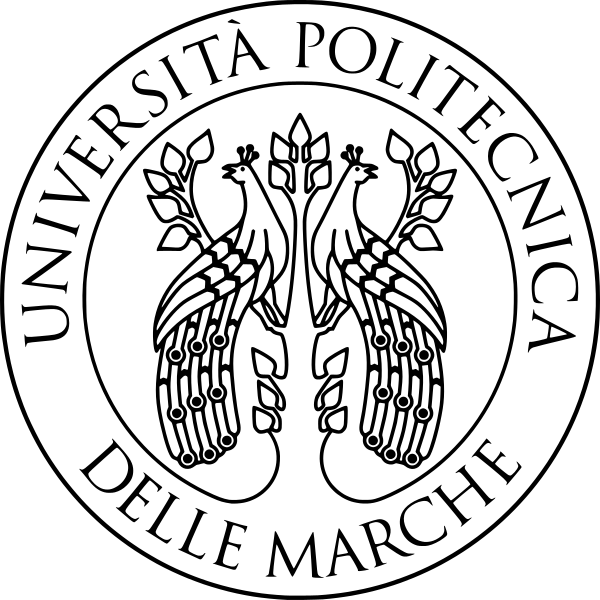
\includegraphics[width=.2\textwidth]{Immagini/univpmlogo}\par\vspace{1cm}
	{\scshape\LARGE Università Politecnica delle Marche\par}
	\vspace{1cm}
	{\scshape\Large Digital Adaptive Circuits And Learning Systems\par}
	\vspace{1.5cm}
	{\huge\bfseries Sound Event Detection con la tecnica del  ``\emph{few-shot learning}''  \par}
	\vspace{2cm}
	{\Large\itshape Matteo Orlandini e Jacopo Pagliuca\par}
	\vfill
	Prof. Stefano \textsc{Squartini}\\
	Dott.ssa Michela \textsc{Cantarini}
	
	\vfill
	
	% Bottom of the page
	{\large \today\par}
\end{titlepage}

\thispagestyle{empty}
\tableofcontents
\clearpage

%\newpage
\setcounter{page}{1}

\section{Introduzione}
\label{section:Introduzione}
\begin{figure}[h]
	\centering	
	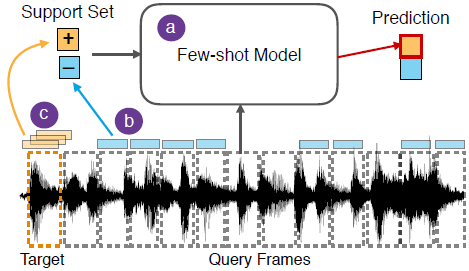
\includegraphics[width=.5\textwidth]{Immagini/few_shot_sound_event_detection_method}
	\caption{Metodo proposto per il few-shot sound event detection. (a) Applicazione del modello few-shot, (b) costruzione del set di esempi negativi, in blu, e (c) data augmentation per la generazioni di più esempi positivi, in arancione.~\cite{Salamon:Few-Shot}}
	\label{fig:few_shot_sound_event_detection_method}
\end{figure}

\begin{figure}[h]
	\centering	
	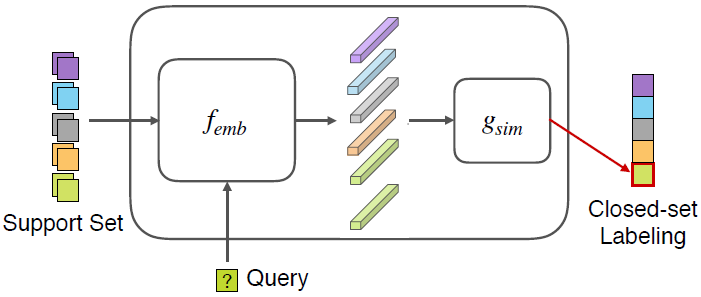
\includegraphics[width=.5\textwidth]{Immagini/few_shot_learning_model}
	\caption{Modello few-shot learning nel caso 5\emph{-way} 2\emph{-shot}.~\cite{Salamon:Few-Shot}}
	\label{fig:few-shot_learning_model}
\end{figure}
\clearpage

\section{Convolutional Neural Network (CNN)}
Una rete neurale convoluzionale è una rete feedforward pensata per applicazioni che richiedono l'elaborazione di immagini o di grandi moli di dati.
L'ingresso della rete è costituito da una o più matrici che attraversano delle fasi di convoluzione che ne riducono le dimensioni. I filtri di convoluzione sono detti kernel o di pooling. Infine, il risultato viene passato a una rete fully connected che ha il compito di classificazione.

La prima parte del filtro consiste nella convoluzione dell'immagine in ingresso con una serie di kernel i cui parametri vengono allenati.
Il filtro viene traslato in entrambe le dimensioni della matrice producendo una serie di feature bidimensionali.
Il parametro \textit{stride} definisce il passo con cui il kernel viene traslato sulla matrice di ingresso.
Solitamente, viene effettuato uno zero-padding sui contorni del volume in modo da poter caratterizzare anche i valori che si trovano ai bordi delle matrici.
In seguito alla convoluzione viene applicata una funzione non-lineare come ad esempio una sigmoide o una ReLu con lo scopo di aumentare la proprietà di non linearità.

Il pooling layer è uno strato della rete che ha lo scopo di ridurre le dimensioni della matrice prodotta dal convolutional layer. Combinando gruppi di elementi della matrice (solitamente 2x2) restituisce il valore massimo tra essi, che andrà a sostituire il blocco stesso.

\section{Area under precision-recall curve (AUPRC)}
Nella fase di test, la rete elabora una predizione dell'output a partire da un ingresso noto che poi viene confrontata con il valore effettivo.
Nel nostro caso è presente un positive set e un negative set, si tratta quindi di classificazione binaria.
Il confronto tra predizione e label può produrre quattro risultati:
\begin{itemize}
	\item Vero Negativo (TN): il valore reale è negativo e il valore predetto è negativo;
	\item Vero Positivo (TP): il valore reale è positivo e il valore predetto	è positivo;
	\item Falso Negativo (FN): il valore reale è positivo e il valore predetto è negativo;
	\item Falso Positivo (FP): il valore reale è negativo e il valore predetto	è positivo;
\end{itemize}
Questi valori vanno a comporre la confusion matrix.
Nel nostro caso siamo interessati a Precision e Recall.

Il parametro Precision rappresenta quanti tra i casi predetti come positivi sono realmente positivi.

Il parametro Recall indica quanti tra i casi realmente positivi è stato predetto in modo corretto.
\begin{equation}
Precision=\frac{TP}{TP+FP}
\end{equation}
\begin{equation}
Recall=\frac{TP}{TP+FN}
\end{equation}
\section{Few-shot learning}
\label{section:Few-shot}
(https://www.borealisai.com/en/blog/tutorial-2-few-shot-learning-and-meta-learning-i/)
\subsection{Introduzione}
Gli esseri umani possono riconoscere nuove classi di oggetti partendo da pochissimi esempi. Tuttavia, la maggior parte delle tecniche di machine learning richiedono migliaia di esempi per ottenere prestazioni simili a quelle umane. L'obiettivo del \emph{few-shot learning} è classificare i nuovi dati dopo aver visto solo pochi esempi di training. Nel caso estremo, potrebbe esserci solo un singolo esempio per ogni classe (\emph{one shot learning}). In pratica, il few-shot learning è utile quando è difficile trovare esempi di training (ad es. casi di una malattia rara) o quando il costo dell'etichettatura dei dati è elevato.

L'apprendimento few-shot viene solitamente studiato utilizzando la classificazione \emph{N-way-K-shot}. L'obiettivo è quello di discriminare le N classi composte da K esempi ciascuna. Una tipica dimensione del problema potrebbe essere quella di discriminare tra $N=10$ classi con solo $K=5$ campioni ciascuno di training. Non possiamo allenare un classificatore usando metodi convenzionali; qualsiasi algoritmo di classificazione moderno dipenderà da molti più parametri rispetto agli esempi di addestramento e generalizzerà male.

Se i dati non sono sufficienti per ridurre il problema, una possibile soluzione è acquisire esperienza da altri problemi simili. A tal fine, la maggior parte degli approcci caratterizza l'apprendimento a breve termine con un problema di meta-apprendimento.

\subsection{The meta learning framework}
Nel framework di apprendimento classico, impariamo come classificare dai dati di training e valutiamo i risultati utilizzando i dati di test. Nel quadro del meta-apprendimento, \textit{impariamo come imparare} a classificare in base a una serie di \textit{training task} e valutiamo utilizzando una serie di test task; In altre parole, usiamo un insieme di problemi di classificazione per aiutare a risolvere altri insiemi non correlati.

Qui, ogni attività imita lo scenario few-shot, quindi per la classificazione N-way-K-shot, ogni attività include N classi con K esempi ciascuna. Questi sono noti come support set per il task e vengono utilizzati per apprendere come risolvere il task. Inoltre, esistono ulteriori esempi delle stesse classi, note come set di query, utilizzate per valutare le prestazioni del task corrente. Ogni task può essere completamente unico; potremmo non vedere mai le classi di un task in nessuno degli altri. L'idea è che il sistema veda ripetutamente istanze (task) durante l'addestramento che corrispondono alla struttura dell'attività finale di few-shot, ma che contengono classi diverse.

Ad ogni fase del meta-apprendimento, aggiorniamo i parametri del modello in base ad un training task selezionato casualmente. La funzione di loss è determinata dalle prestazioni di classificazione sul set di query del task, in base alla conoscenza acquisita dal relativo set di supporto. Poiché la rete viene sottoposta ad un compito diverso in ogni fase temporale, deve imparare a discriminare le classi di dati in generale, piuttosto che un particolare sottoinsieme di classi.

Per valutare le prestazioni in pochi colpi, utilizziamo una serie di attività di test. Ciascuno contiene solo classi invisibili che non erano in nessuna delle attività di formazione. Per ciascuno, misuriamo le prestazioni sul set di query in base alla conoscenza del loro set di supporto.

\subsection{Approcci al meta-apprendimento}
Gli approcci al meta-apprendimento sono diversi e non c'è consenso sull'approccio migliore. Tuttavia, esistono tre famiglie distinte, ognuna delle quali sfrutta un diverso tipo di conoscenza a priori:
\begin{itemize}
	\item Conoscenze a priori sulla somiglianza: apprendiamo degli embedding nei training task che tendono a separare classi diverse anche quando non sono visibili.
	\item Conoscenze a priori sull'apprendimento: utilizziamo le conoscenze a priori per vincolare l'algoritmo di apprendimento a scegliere parametri che generalizzino bene da pochi esempi.
	\item Conoscenza a priori dei dati: sfruttiamo le conoscenze a priori sulla struttura e la variabilità dei dati e questo ci consente di apprendere modelli praticabili da pochi esempi.
\end{itemize}

\section{Prototypical Network}
L'approccio si basa sull'idea che esiste un embedding in cui i punti delle istanze di una classe si raggruppano attorno a una singola rappresentazione prototipo per ogni classe.
Nella classificazione few-shot per ogni episodio viene fornito un support set di $N$ esempi etichettati  $S=\{(\mathbf{x}_1,y_1), \dots,(\mathbf{x}_N,y_N)\}$ dove $\mathbf{x}_i\in \mathbb{R}^D$ rappresenta il vettore $D$-dimensionale della feature (nel nostro caso spettrogrammi di dimensione $128 \times 51$) e $y_i \in \{1, \dots, K\}$ la rispettiva label. $S_k$ denota il set di esempi etichettati con la classe $k$.

La rete Prototypical calcola una rappresentazione $M$-dimensionale $\mathbf{c}_k$, o \emph{prototipo}, di ogni classe tramite una funzione di embedding $f_\phi : \mathbb{R}^D \rightarrow \mathbb{R}^M$ con parametri da allenare $\phi$. La funzione di embedding è rappresentata da una rete convoluzionale. Ogni prototipo è il vettore media tra gli embedding delle istanze della stessa classe.
\begin{equation}
	\mathbf{c}_k=\frac{1}{|S_k|}\sum_{(\mathbf{x}_i,y_i)\in S_k}f_\phi (\mathbf{x}_i)
\end{equation}
Data una funzione distanza $d: \mathbb{R}^M \times \mathbb{R}^M \rightarrow [0, +\infty )$, la rete Protypical calcola la relazione di una query $\mathbf{x}$ rispetto ai prototipi tramite la funzione softmax delle distanze prese con segno negativo.
\begin{equation}
p_\phi(y=k|\mathbf{x})=\dfrac{\exp(-d(f_\phi(\mathbf{x}),\mathbf{c}_k))}{\sum_k' \exp(-d(f_\phi(\mathbf{x}),\mathbf{c}_k'))}
\end{equation}
Il processo di training avviene minimizzando il negativo del logaritmo della probabilità $J(\phi)=-\log\left(p_\phi(y=k|\mathbf{x})\right)$ considerando la distanza fra query e il prototipo della sua classe.
Gli episodi di training sono formati campionando C classi di parole da un lettore e selezionando per ognuna casualmente K istanze e Q query.

\begin{figure}[h]
	\centering
	\subfloat[Few-shot\label{fig:proto_few_shot}]{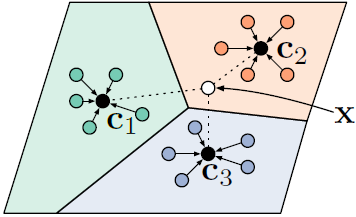
\includegraphics[width=0.3\textwidth]{Immagini/proto_few_shot}}
	\qquad
	\subfloat[Zero-shot\label{fig:proto_zero_shot}]{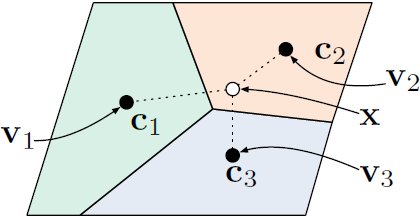
\includegraphics[width=0.35\textwidth]{Immagini/proto_zero_shot}}
	\label{fig:proto_few_zero_shot}	
	\caption{Reti Prototypical negli scenari few-shot e zero-shot. (a): i prototipi few-shot $\mathbf{c}_k$ sono calcolati come la media degli embedding del support set per ogni classe. (b): i prototipi zero-shot $\mathbf{c}_k$ sono prodotti facendo l'embedding dei metadati $\mathbf{v}_k$. In entrambi i casi i punti degli embedding delle query sono classificati facendo il softmax sulle distanze del prototipo delle classi: $p_\phi(y = k|\mathbf{x}) \propto \exp \left(-d(f_\phi(\mathbf{x}),\mathbf{c}_k) \right)$.~\cite{snell:prototypical}}
\end{figure}
\clearpage

\section{Relation Network}
La rete Relation ha lo scopo di associare due istanze alla volta per determinare la loro similarità.
Questo viene effettuato concatenando gli embedding di più istanze in un unico elemento che sarà dato in ingresso a una rete decisionale i cui parametri saranno aggiornati in modo che una concatenazione di elementi simili restituisca un risultato vicino a 1.
La Relation Network è costituita da due moduli: un modulo di \emph{embedding} $f_\varphi$ (equivalente a quello nella Prototypical) e un modulo di \emph{relation} $g_\phi$, come illustrato in figura~\ref{fig:relation_network}.
Le istanze $x_i$ del query set $\mathcal{Q}$ e quelle $x_j$ del support set $\mathcal{S}$ vengono date in ingresso al modulo di embedding producendo dei vettori (feature maps) $f_\varphi(x_i)$ e $f_\varphi(x_j)$.
Questi ultimi vengono poi dati all'operatore $\mathcal{C}(\cdot ,\cdot)$ che ne fa la concatenazione: $\mathcal{C}(f_\varphi(x_i),f_\varphi(x_j))$.
Le feature map concatenate passano poi attraverso il modulo di decisione che restituisce uno scalare da 0 a 1, il quale rappresenta la somiglianza tra $x_i$ e $x_j$.
Per il caso $C$-way one-shot, viene concatenata la query con le istanze delle $C$ classi producendo $C$ punteggi di somiglianza.
\begin{equation}
	r_{i,j}=g_\phi(\mathcal{C}(f_\varphi(x_i),f_\varphi(x_j))),  \qquad i = 1, 2, \dots, C
\end{equation}
Nel caso $C$-way K-shot invece, la query viene concatenata con la somma elemento per elemento degli embedding di ogni istanza delle classi. Quindi, in entrambi i casi i confronti $r_{i,j}$ sono $C$ per ogni query.

Per allenare il modello viene usato l'errore quadratico medio (MSE) in modo che l'uscita del modulo di decisione produca 1 se i vettori concatenati sono della stessa classe e 0 altrimenti.

\begin{figure}[h]
	\centering	
	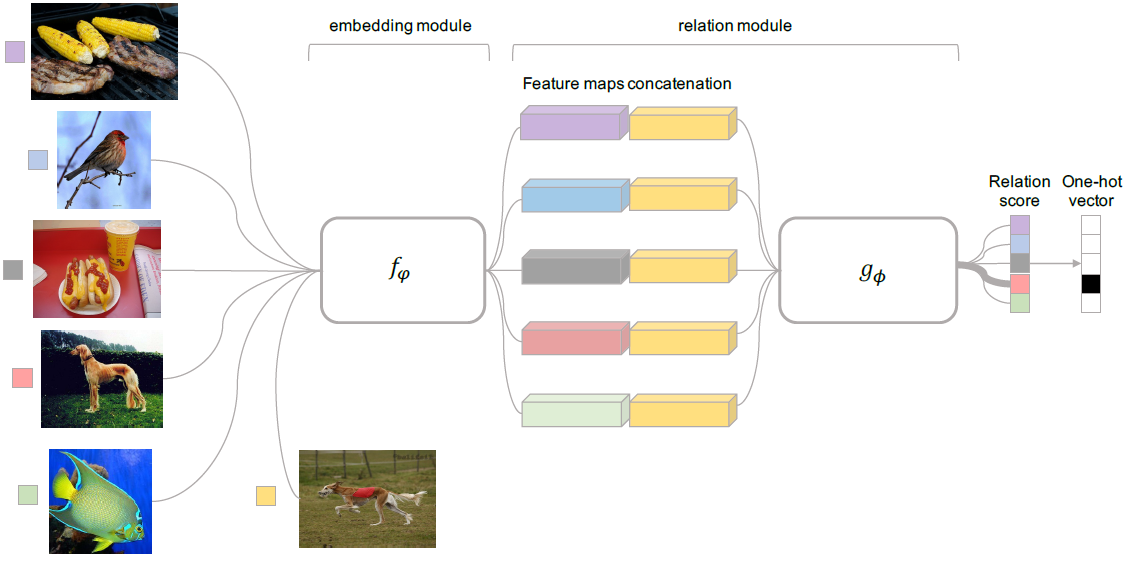
\includegraphics[width=.8\textwidth]{Immagini/relation_network}
	\caption{Architettura della Relation Network nel caso 5\emph{-way} 1\emph{-shot} con un esempio di query.~\cite{DBLP:journals/corr/abs-1711-06025}}
	\label{fig:relation_network}
\end{figure}

\begin{figure}[h]
	\centering
	\subfloat[Blocco convoluzionale\label{fig:relation_network_architecture_a}]{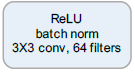
\includegraphics[width=0.3\textwidth]{Immagini/relation_network_conv_block}}
	\qquad
	\subfloat[Relation Network per few-shot learning\label{fig:relation_network_architecture_b}]{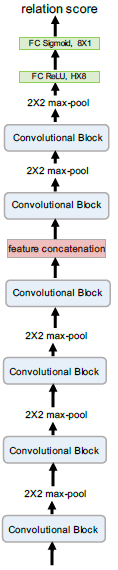
\includegraphics[width=0.3\textwidth]{Immagini/relation_network_architecture}}
	\label{fig:relation_network_architecture}	
	\caption{Architettura della Relation Network per few-shot learning (b) composta dagli elementi inclusi nel blocco convoluzionale (a).~\cite{DBLP:journals/corr/abs-1711-06025}}
\end{figure}

\clearpage

\section{Dataset Spoken Wikipedia Corpora}
\label{sec:spoken_wikipedia_corpora}
Il progetto Spoken Wikipedia unisce lettori volontari di articoli di Wikipedia. Sono disponibili centinaia di articoli in inglese, tedesco e olandese per gli utenti che non sono in grado o non vogliono leggere la versione scritta dell'articolo. Il dataset trasforma i file audio in un corpus, cioè una raccolta ordinata e completa di opere o di autori, allineato nel tempo, rendendolo accessibile per la ricerca.\cite{minining_spoken_wikipedia}

Questo corpus ha diverse caratteristiche importanti:
\begin{itemize}
	\item centinaia di ore di audio allineato
	\item lettori eterogenei
	\item diversi argomenti
	\item genere testuale ben studiato
	\item le annotazioni delle parole possono essere mappate all'html originale
	\item allineamenti a livello di fonema
\end{itemize}

Ogni articolo è suddiviso in sezioni, frasi e token. Ogni token è normalizzato e la normalizzazione è allineata all'audio.

\subsection{Annotazioni}
Ogni annotazione è racchiusa in un tag chiamato ``\texttt{article}'', che contiene una sezione ``\texttt{meta}'' per i metadati, come si può vedere in~\ref{metadati_annotazioni} e una sezione ``\texttt{d}'', come in~\ref{annotazioni}, contenente l'articolo e le relative annotazioni.

\label{subsec:annotazioni}
\begin{lstlisting}[language=XML,firstnumber=1, caption=Metadati delle annotazioni delle parole in un audio, label=metadati_annotazioni,captionpos=b]
<article>
	<meta>
		<link key="DC.conformsto" value="http://nats.gitlab.io/swc/schema/swc-1.0.rnc"/>
		<prop key="DC.creator" value="Spoken Wikipedia Corpus Collection Software"/>
		<prop key="DC.publisher" value="Universität Hamburg"/>
		<link key="DC.reference" value="http://nbn-resolving.de/urn:nbn:de:gbv:18-228-7-2209"/>
		<prop key="DC.type" value="dataset"/>
		<prop key="DC.license" value="CC-BY-SA"/>
		<prop key="DC.title" value="Limerence"/>
		<prop key="DC.language" value="en"/>
		<prop key="DC.identifier" value="Limerence"/>
		<prop key="DC.date.read" value="2005-04-29 00:00:00"/>
		<link key="DC.source" value="https://en.wikipedia.org/wiki/Limerence"/>
		<prop key="DC.source.wikiID" value="154147"/>
		<prop key="DC.source.revision" value="791627969"/>
		<link key="DC.source.text" value="https://en.wikipedia.org/w/index.php?title=Limerence&oldid=13811989"/>
		<link key="DC.source.audio" value="https://upload.wikimedia.org/wikipedia/commons/a/aa/Limerence.ogg" group="audio1"/>
		<prop key="DC.source.audio.offset" value="0.0" group="audio1"/>
		<link key="DC.source.audio.page" value="https://en.wikipedia.org/w/index.php?title=File%3aLimerence.ogg" group="audio1"/>
		<link key="DC.source.audio.date" value="2007-09-14 19:23:05" group="audio1"/>
		<prop key="reader.name" value="the Epopt"/>
		<prop key="processing.step" value="tokenize" group="tokenize"/>
		<prop key="processing.step.date" value="2017-08-10T07:44:44.095+02:00[Europe/Berlin]" group="tokenize"/>
		<prop key="processing.step.options" value="Namespace(output=articles/Limerence/tokenized.swc, all_sections=false, null_normalize=false, raw_output=null, subparser_name=tokenize, lang=en, no_introduction=false, article_dir=articles/Limerence)" group="tokenize"/>
		<prop key="processing.step.git.commit.id" value="7431dbf93f212ad828208abaf8f518fb8de11ff3" group="tokenize"/>
		<prop key="processing.step.git.commit.time" value="09.08.2017 @ 15:21:55 CEST" group="tokenize"/>
		<prop key="processing.step" value="align" group="align"/>
		<prop key="processing.step.date" value="2017-08-11T16:12:18.423+02:00[Europe/Berlin]" group="align"/>
		<prop key="processing.step.options" value="Namespace(output=articles/Limerence/aligned.swc, transcript=articles/Limerence/tokenized.swc, g2p=../model_en/model.fst.ser, phone=false, subparser_name=align, dict=../model_en/empty.dic, acoustic_model=../model_en/, audio=articles/Limerence/audio.wav)" group="align"/>
		<prop key="processing.step.git.commit.id" value="7431dbf93f212ad828208abaf8f518fb8de11ff3" group="align"/>
		<prop key="processing.step.git.commit.time" value="09.08.2017 @ 15:21:55 CEST" group="align"/>
	</meta>
\end{lstlisting}
Il documento, contrassegnato dal tag ``\texttt{d}'', può contenere parti diverse, ciascuna spiegata di seguito. La sezione ``\texttt{extra}'' contiene il testo che abbiamo incluso ma non fa parte dell'articolo, ``\texttt{ignored}'' contiene ciò che fa parte del testo ma viene ignorato per l'allineamento, ``\texttt{section}'' contiene un titolo e un contenuto, ``\texttt{p}'' contiene un paragrafo  e ``\texttt{s}'' una frase che a sua volta contiene dei token ``\texttt{t}''. In quest'ultimo è contenuta la singola parola originale e le normalizzazioni. Per esempio, la punteggiatura non ha annotazioni di normalizzazione in quanto non è pronunciata, ma il numero 500 ne ha due - ``cinque'' e ``cento''. un token stesso non ha allineamento, solo la sua normalizzazione ``\texttt{n}'' è allineata. La normalizzazione ha una ``\texttt{pronunciation}'' e può avere un tempo di ``\texttt{start}'' ed ``\texttt{end}'', se è allineata. La normalizzazione, a sua volta, può contenere dei fonemi ``\texttt{ph}''.

\begin{lstlisting}[language=XML,firstnumber=1, caption=Annotazioni delle parole in un audio, label=annotazioni,captionpos=b]
<d>
	<extra text="LimerenceFrom wikipedia, the free encyclopedia at e n dot wikipedia dot org.">
		<s text="LimerenceFrom wikipedia, the free encyclopedia at e n dot wikipedia dot org.">
			<t text="LimerenceFrom">
				<n pronunciation="LimerenceFrom" start="140" end="1190"/>
			</t>
			<t text="wikipedia">
				<n pronunciation="wikipedia" start="1250" end="1950"/>
			</t>
			<t text=","/>
			<t text="the">
				<n pronunciation="the" start="1950" end="2070"/>
			</t>
			<t text="free">
				<n pronunciation="free" start="2070" end="2300"/>
			</t>
			<t text="encyclopedia">
				<n pronunciation="encyclopedia" start="2300" end="3220"/>
			</t>
			<t text="at">
				<n pronunciation="at"/>
			</t>
			<t text="e">
				<n pronunciation="e" start="3490" end="3710"/>
			</t>
\end{lstlisting}

\subsection{Lettori}
\label{subsec:lettori}
Il dataset Spoken Wikipedia Corpora contiene un totale di 1340 audio di diversi lettori, ma nel progetto vengono presi solo gli audio che contengono annotazioni a livello di parola. In questo modo vengono presi solo 208 lettori e partizionati come in~\cite{Salamon:Few-Shot} con un rapporto $138:15:30$ tra lettori di training, validation e test. I lettori e le parole sono state estratte dai file ``aligned.swc'' contenuti in ogni audio e, successivamente, salvati in diversi file json. Per la gestione dei json sono state create due funzioni utili per la lettura e scrittura come mostrato nel codice~\ref{json_manager}.
\begin{lstlisting}[language=iPython,firstnumber=1, caption=json\_manager.py, label=json_manager,captionpos=b]
import json
	
def write_json_file(filename, list_of_dict, indent = 0):
	f = open(filename, "w")
	f.write(json.dumps(list_of_dict, indent = indent))
	f.close
	
def read_json_file(filename):
	f = open(filename, "r")
	list_of_dict = json.load(f)
	f.close
	return list_of_dict
\end{lstlisting}

Il codice~\ref{xml_parser_readers} salva un file json chiamato ``readers\_paths.json'' formato dalle chiavi ``reader\_name'' e ``folder'' i cui valori sono rispettivamente il nome del lettore e le cartelle in cui sono salvati i file audio registrati dal relativo lettore, come si può vedere nel json~\ref{JSON_lettori}. Questo codice, usando la libreria \texttt{xml.etree.ElementTree} e la funzione \texttt{ET.parse}, rappresenta l'intero documento XML come un albero. La funzione \texttt{getroot} ne trova la radice e, successivamente, si scorre l'albero iterando finché non si trova il tag ``\texttt{prop}'' in cui è contenuta la chiave ``\texttt{reader.name}''. Inoltre, si effettua un controllo sul nome del lettore perché può capitare che viene salvato nel file ``aligned.swc'' con nomi diversi. Ad esempio, in alcuni file si può trovare nella chiave ``reader.name'' il valore ``:en:user:alexkillby|alexkillby'', mentre in altri solo ``alexkillby'' oppure si può trovare ``user:popularoutcast'', mentre in altri solo ``popularoutcast''. Una volta noto il nome del lettore si vede se è già presente nella lista di dizionari e se è un lettore nuovo lo si aggiunge con il relativo nome del file audio, mentre se il lettore era già presente si aggiunge solamente il nome del file audio.

\begin{lstlisting}[language=iPython,firstnumber=1, caption=xml\_parser\_readers.py, label=xml_parser_readers,captionpos=b]
import xml.etree.ElementTree as ET
from tqdm import tqdm
import os
import json
from json_manager import *

# Initialize list with empty dictionaries
readers = []

source_path = "./Dataset/English spoken wikipedia/english/"
filename = "aligned.swc"

# search for readers for each folder
for audio_path in os.scandir(source_path):
	# save only folder name from entire path
	folder =  os.path.basename(audio_path)
	if (os.path.exists(source_path + "/" + folder + "/" + filename)):
		# parse the xml file "aligned.swc"
		tree = ET.parse(source_path + "/" + folder + "/" + filename)
		# getroot returns the root element for this tree
		root = tree.getroot()
		#root.iter creates a tree iterator with the current element as the root.
		# The iterator iterates over this element and all elements below it, in 
		# document (depth first) order.
		for property in root.iter(tag = 'prop'):
			# if the key "reader.name" exists
			if (property.attrib['key'] == 'reader.name'):
				# save the reader name taking the value of the attribute
				reader_name = property.attrib['value'].lower()
				# fix readers names that contain "user:"
				if ("user:" in reader_name):
				# fix readers names that contain "|""
					if ("|" in reader_name):
						# example reader_name = [[:en:user:alexkillby|alexkillby]] -> 
						# reader_name = alexkillby
						reader_name = reader_name[reader_name.find("user:")+5:reader_name.find("|")]
						# fix readers names that contain "|""
					elif ("]]" in reader_name):
						# example reader_name = [[user:popularoutcast]] -> 
						# reader_name = popularoutcast
						reader_name = reader_name[reader_name.find("user:")+5:reader_name.find("]]")]
				# if the reader is not yet on the list create a dict and append to
				# the readers list
				if not any(reader['reader_name'] == reader_name for reader in readers):
					dictionary = {'reader_name': reader_name, 'folder' : [folder]}
					readers.append(dictionary)
				else:
					# if the reader is already on the list add the folder name
					for reader in readers:
						if (reader['reader_name'] == reader_name):
							reader['folder'].append(folder)
# print the number of the readers
print("The readers are:", str(len(readers)))

# save a "readers_paths.json" with the name of the readers and the relative
# file audio folders
write_json_file("readers_paths.json", readers, indent = 4)
\end{lstlisting}

\begin{lstlisting}[language=json,firstnumber=1, caption=Formato del file readers\_paths.json, label=JSON_lettori,captionpos=b]
{
	"reader_name": "the epopt",
	"folder": [
		"(I_Can%27t_Get_No)_Satisfaction",
		"Ceremonial_ship_launching",
		"Limerence",
		"Revolt_of_the_Admirals",
		"Ship_commissioning"
	]
},
{
	"reader_name": "wodup",
	"folder": [
		"0.999..%2e",
		"Execution_by_elephant",
		"Hell_Is_Other_Robots",
		"Tom_Bosley",
		"Truthiness"
	]
},
\end{lstlisting}

\subsection{Parole}
\label{subsec:parole}
Il codice~\ref{find_target_words}..............................

\begin{lstlisting}[language=iPython,firstnumber=1, caption=find\_target\_words.py, label=find_target_words,captionpos=b]
import xml.etree.ElementTree as ET
from tqdm import tqdm
import os
import collections
from json_manager import *
import random

folder = []
source_path = "./Dataset/English spoken wikipedia/english/"
filename = "aligned.swc"
file_audio_name = "audio.ogg"

# iterate in each folder of the dataset
for folder in tqdm(os.scandir(source_path), desc = "Folder number"):
    # initialize the list of dict "target_words"
    target_words = []
    if (os.path.exists(folder.path + "/" + filename) \
        and os.path.exists(folder.path + "/" + file_audio_name) \
        and os.path.isdir(folder.path)):  
        # parse the xml file aligned.swc
        tree = ET.parse(folder.path + "/" + filename)
        # getroot returns the root element for this tree
        root = tree.getroot()
        # initialize the list "words"
        words = []
        # root.iter creates a tree iterator with the current element as the 
        # root. The iterator iterates over this element and # all elements 
        # below it, in document (depth first) order.
        for token_normalization in root.iter(tag = 'n'):
            # we take only the words with the timestamp, so only if there is
            # 'start' (or 'end') tag
            if 'start' in token_normalization.keys():
                # add every word with "start" key
                words.append(token_normalization.attrib['pronunciation'].lower())
        # collections.Counter stores elements as dictionary keys, and their
        # counts are stored as dictionary values.
        unique_words = collections.Counter(words)
        # for each key (word) in "unique_words" append a new target_word if
        # the number of occurency is at least 10
        for key in unique_words.keys():
            # we only consider words that occur at least 10 times in the
            # recording. Note that unique_words[key] is the word frequency
            if (unique_words[key] >= 10):
                # add a new target word
                target_words.append({'word' : key, \
                                     'frequency' : unique_words[key], \
                                     'start' : [], \
                                     'end' : []})
        # for each "target_words" append the relative "start" and "end"
        # timestamp
        for token_normalization in root.iter(tag = 'n'):
            # we take only the words with the timestamp, so only if there is 'start' (or 'end') tag
            if 'start' in token_normalization.keys():
                # iterate over the "target_words"
                for target_word in target_words:
                    # add start and end timestamp only to the relative
                    # "target_word"
                    if target_word['word'] == token_normalization.attrib['pronunciation'].lower():
                        target_word['start'].append(int(token_normalization.attrib['start']))
                        target_word['end'].append(int(token_normalization.attrib['end']))

        write_json_file(folder.path+"/word_count.json", target_words, indent = 4)
        # If there are more than 10 words that occur at least 10 times in
        # the recording, we sort the words by their number of occurrences,
        # divide the sorted list into 10 equally sized bins, and sample 
        # one keyword per bin.
        if (len(target_words) >= 10):
            target_words = random.sample(target_words, 10)
        # save the "target_words.json"
        write_json_file(folder.path+"/target_words.json", target_words, indent = 4)

\end{lstlisting}

\begin{lstlisting}[language=json,firstnumber=1, caption=Formato del file word\_count.json, label=word_count,captionpos=b]
{
        "word": "i",
        "frequency": 12,
        "start": [
            660,
            8800,
            115050,
            ...
        ],
        "end": [
            870,
            8940,
            115240,
            ...
        ]
    },
    {
        "word": "the",
        "frequency": 75,
        "start": [
            4160,
            49930,
            53680,
            ...
        ],
        "end": [
            4320,
            50030,
            53710,
			...
   		]                
    },
\end{lstlisting}
            
Il file ``readers\_paths.json'' viene successivamente usato per salvare le parole di ogni lettore, il nome della relativa cartella in cui vengono pronunciate e i timestamp di inizio e fine della parola per ogni cartella come mostrato nel json~\ref{readers_words}. Il codice~\ref{words_per_reader} legge il nome di ogni lettore dal json precedentemente salvato, successivamente per ognuna delle cartelle del lettore si....................................

\begin{lstlisting}[language=iPython,firstnumber=1, caption=words\_per\_reader.py, label=words_per_reader,captionpos=b]
from tqdm import tqdm
import os
from json_manager import *

source_path = "./Dataset/English spoken wikipedia/english/"
# read the json that contains the readers name and their audio folders
readers = read_json_file("readers_paths.json")
#initialize a list of dict
readers_words = []
# for each reader search the word spoken by the reader
for reader in tqdm(readers):
    # create a dict with 'reader_name' and 'words' keys
    new_readers_words = {'reader_name' : reader['reader_name'],\
                         'words' : [] }

    # for each reader create a new dict for words
    words_per_reader = [] 
    # flag to signal if "word_count.json" exists
    json_file_exist = False
    # search for each folder the file "word_count.json"
    for reader_folder in reader['folder']:
        if (os.path.exists(source_path + "/" + reader_folder + "/word_count.json")):
            # "word_count.json" exists
            json_file_exist = True
            # read "word_count.json"
            recording_words = read_json_file(source_path + "/" + reader_folder + "/word_count.json")
            # for each audio folder create a new list of dict
            folder_per_word = []
            # for each word in the audio save the folder, start and end 
            # timestamps
            for word in recording_words:
                 # create a dict with 'folder', 'start' and 'end' keys
                folder_per_word = {'folder' : reader_folder, \
                                   'start' : word['start'], \
                                   'end' : word['end']}
                # if the word is not yet in the list add the word
                if not any (word['word'] == word_per_reader['word'] for word_per_reader in words_per_reader):
                   words_per_reader.append({ 'word' : word['word'], \
                                             'folders' : [folder_per_word]}) \
                # otherwise add 'start' and 'end' if the "reader_folder" is 
                # in word_per_reader['folders'] or add the "folder_per_word"  
                else:
                    for word_per_reader in words_per_reader:
                        if word['word'] == word_per_reader['word']:
                            if reader_folder in word_per_reader['folders']:
                                for folder in word_per_reader['folders']:
                                    if reader_folder == folder['folder']:
                                        folder['start'] += word['start']
                                        folder['end'] += word['end']
                            else:
                                word_per_reader['folders'].append(folder_per_word)
    # if "word_count.json" exists add the new reader to "training_readers"
    # list     
    if (json_file_exist):
        new_readers_words['words'] = words_per_reader
        readers_words.append(new_readers_words)
# save a "readers_words.json" with the name of the readers and the relative 
# words spoken
write_json_file("readers_words.json", readers_words, indent = 0)

\end{lstlisting}
	
\begin{lstlisting}[language=json,firstnumber=1, caption=Formato del file readers\_words.json, label=readers_words,captionpos=b]
"reader_name": "wodup",
		"words": [
			{
				"word": "the",
				"folders": [
					{
						"folder": "0.999..%2e",
						"start": [
							6950,
							1029740,
							1032520,
							...
						],
						"end": [
							7190,
							1029880,
							1032620,
							...
						]
					},
					{
						"folder": "Execution_by_elephant",
						"start": [
							3600,
							10680,
							...
\end{lstlisting}



\section{Protonet codice}
\subsection{Protonet training}
La funzione \texttt{get\_training\_validation\_readers}, a partire dalla lista di lettori di training/validation, seleziona quelli che hanno almeno un numero di parole diverse pari a C e li suddivide tra training e validation seguendo il rapporto usato in [ARTICOLO RIFERIMENTO]: 138/153 e 15/153.
Per fare ciò scorre l'elenco delle directory dei lettori e salva su un array le parole a loro associate. Al termine di questa operazione, se il numero di parole è almeno C il lettore è ritenuto valido e il suo nome viene aggiunto a una lista. Infine la lista viene scissa come spiegato sopra.


Il primo for rappresenta l'inizio degli episodi.
Il numero totale di iterazioni è 60000 come in [ARTICOLO]; per ogni episodio viene richiamata la funzione \texttt{batch\_sample}.
Essa campiona a caso uno dei lettori di training e di questo seleziona casualmente C parole.
Per ognuna di queste parole si ricava il numero di istanze presenti del dataset.
Viene inizializzato un vettore con gli indici di queste e ne vengono campionati K+Q in \texttt{index}. Poi, iterando, gli spettrogrammi il cui indice è presente in \texttt{index} vengono salvati e divisi in K istanze del support set e Q istanze del query set.


Una volta ottenute, le feature del support set e query set vengono date in ingresso alla funzione \texttt{loss}.
Queste ultime vengono messe in fila e concatenate per poter essere passate al modello che calcolerà gli embedding per ogni istanza.
Gli elementi del support set che fanno parte della stessa classe andranno a costituire i prototipi tramite una media dei loro valori: \texttt{prototypes = embeddings[:n\_class*n\_support].view(n\_class, n\_support, embeddings\_dim).mean(1)}.


Il parametro \texttt{target\_inds} viene costruito ripetendo l'indice di ogni classe per il numero di query e sarà utilizzato per poter ricordare a che classe appartiene ogni query.

Per ogni elemento del query set vengono calcolate le distanze rispetto ai prototipi di ogni classe tramite la funzione \texttt{euclidean\_dist} che rappresenta la distanza euclidea.
Per ogni query viene poi usata la funzione di attivazione \texttt{log\_softmax} fra tutte le sue distanze.
La funzione loss da minimizzare è costituita dalla media dei \texttt{log\_softmax} della classe corrispondente alla query presi con segno negativo. Infatti, nel caso ideale in cui la distanza delle query della stessa classe dal prototipo è 0, la media dei softmax delle distanze dal prototipo assegnato sarà nulla.
La accuracy invece è determinata dal numero dei casi in cui il prototipo a distanza minima da una query (o il massimo del softmax) corrisponde con il prototipo della classe associata alla query.


Con \texttt{loss\_out.backward()} viene utilizzata la loss per la retropropagazione che aggiorna i parametri della rete.
\subsection{Protonet validation}
Ogni 5000 episodi del training vengono effettuati 1000 episodi di validation.
Come nel training vengono ricavati support set e query set ma in questo caso dai lettori di validation.
Per questi vengono calcolati con la funzione \texttt{loss} allo stesso modo loss e accuracy e vengono salvati.
In questo caso però i parametri del modello non vengono aggiornati.
Questo processo è necessario per verificare l'effettività del modello su ingressi mai visti in fase di training.
Al termine dei 1000 episodi di validation, se la media dell'accuracy è migliore di quella calcolata nel batch precedente il modello viene salvato e sovrascritto al precedente, altrimenti viene ignorato.
In questo modo si aggira il problema dell'overfitting fungendo da pseudo early stopping. 
\subsection{Protonet test}
Nella fase di test, seguendo l'articolo di riferimento, l'oggetto di interesse non sono i lettori come nel caso di training e validation. Vengono infatti presi in considerazione i singoli audio. Da questi sarà necessario identificare un gruppo di istanze di una parola (il positive\_set) e, campionando nell'audio, si potrà verificare se la rete è in grado di riconoscere la parola designata.


Per ogni audio quindi viene ricavato il numero di parole con spettrogramma (in base al contenuto di Test\_features).
Per ognuna di esse viene ricavato un positive set e un negative set con i quali è possibile verificare la rete.
Questo processo viene ripetuto 10 volte come in [ARTICOLO] in modo da generalizzare il più possibile il test.
Infatti il positive set è  ricavato campionando casualmente p istanze della parola che si sta analizzando, mentre il negative set è ottenuto campionando n istanze fra tutte le altre parole dello stesso audio.
Per fare questo viene usata la funzione \texttt{get\_negative\_positive\_query\_set}.
Tramite un indice che indica le istanze della parola "positiva" vengono campionati p spettrogrammi che vanno a costituire il positive set. Le restanti istanze della stessa parola vengono inserite invece nel query set come esempio di spettrogramma che la rete dovrebbe riconoscere.
Tra l'elenco delle parole viene quindi rimossa la parola postiva con \texttt{words.remove(pos\_word)}.
Usando le restanti vengono ricavate n esempi di negative set campionando a caso una delle parole e una delle istanze di essa.
Allo stesso modo viene formata la seconda metà del query set che rappresenta gli esempi negativi. Il numeri di query negative viene preso uguale a quello delle positive.


A questo punto, i tre set e il modello sono parametri della funzione \texttt{test\_loss}.
Allo stesso modo di training e validation vengono calcolati gli embedding per ogni istanza e i prototipi delle due classi: positive set e negative set.
Vengono calcolate le distanze che sono passate con segno negativo alla funzione \texttt{log\_softmax}.
Tra i risulati viene selezionato il maggiore che rappresenta la predizione della rete: ovvero la classe a cui viene assegnata la query.
Queste predizioni sono contenute nel vettore \texttt{y\_pred\_tmp}, mentre in \texttt{y\_true\_tmp} sono presenti le label reali di ogni query.

Prima di essere utilizzati per calcolare precision e recall, questi due vettori vengono sottoposti a una operazione di complemento a 2 che inverte 0 e 1 in quanto la funzione \texttt{precision\_recall\_curve} richiede che con la label 1 sia identificata la classe positiva.
Infine, \texttt{sklearn.metrics.auc} calcola la AUPRC.
Questo calcolo avviene al termine delle operazioni per ogni audio.
Una volta terminati gli audio viene calcolata media e varianza degli AUPRC.

\clearpage
\nocite{*}
%Il comando \printbibliography produce la sezione bibliografica con relativi
%titolo e testatina. Per mandarne il relativo titolo nell’indice generale si
%usa l’istruzione:
\printbibliography
\end{document} 